Quando esta dissertação teve início o projeto \acrshort{clav} já tinha cerca de 2 anos de desenvolvimento. Assim nesta secção será apresentado o estado da arte do \acrshort{clav} quando esta dissertação iniciou aprofundando principalmente os pontos mais importantes sobre o tema desta dissertação.

\section{Conceitos}
%TODO
TODO
O que é a a classificação e a avaliação
o que é um processo de negócio
exemplos

\section{Iniciativas Semelhantes à CLAV}
%TODO
TODO

\section{Estrutura}
A \acrshort{clav} está dividida em duas partes:
\begin{itemize}
    \item interface (\textit{front-end}) presente em \url{http://clav.dglab.gov.pt}
    \item \acrshort{api} de dados (\textit{back-end} que inclui também duas bases de dados, \textit{GraphDB} e \textit{MongoDB}) presente em \url{http://clav-api.dglab.gov.pt}.
\end{itemize}

Cada parte encontra-se numa máquina diferente.

Através da figura~\ref{fig:clav_struct} é possível ver o possível fluxo tanto de um utilizador a aceder à interface como a de um utilizador a aceder diretamente à \acrshort{api} de dados. No primeiro caso, quando um utilizador acede o servidor da interface da \acrshort{clav} é descarregado para o lado do utilizador o ficheiro \acrshort{html} (\textit{index}) e os vários ficheiros \textit{JavaScript}, \acrshort{css} e \textit{assets} (como imagens, \acrshort{pdf}s, etc) quando necessários. O servidor da interface é nada mais que um servidor \textit{web} com recurso ao \textit{Nginx} que hospeda estes ficheiros, os quais representam a interface construída com o \textit{Vue} e o \textit{Vuetify}. Como tal o código apresenta-se todo do lado do utilizador e os pedidos à \acrshort{api} serão feitos do computador do utilizador para o servidor da \acrshort{api} de dados e não do servidor da interface para o servidor da \acrshort{api} de dados. Ou seja, o fluxo de cada um desses pedidos será igual ao fluxo no caso em que se acede diretamente a \acrshort{api} sem uso de qualquer interface.

\begin{figure}[H]
    \begin{center}
        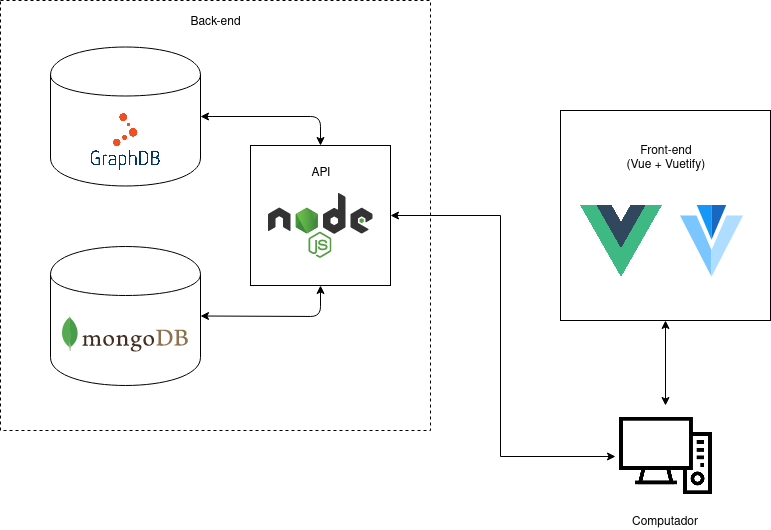
\includegraphics[width=0.7\textwidth]{img/clav_struct.png}
    \end{center}
    \caption{Estrutura da \acrshort{clav} incluindo a interação de um utilizador com a mesma}\label{fig:clav_struct}
\end{figure}

Esta estrutura evoluiu depois para a estrutura presente na figura~\ref{fig:clav_struct2} em que tanto a interface como o \textit{back-end} estão ``por trás'' do \textit{Nginx} o que leva a que todos os pedidos passem por este, seja para obter a interface (onde o \textit{Nginx} devolve esta) como para aceder a \acrshort{api} de dados (onde o \textit{Nginx} reencaminha o pedido para a \acrshort{api}).

\begin{figure}[H]
    \begin{center}
        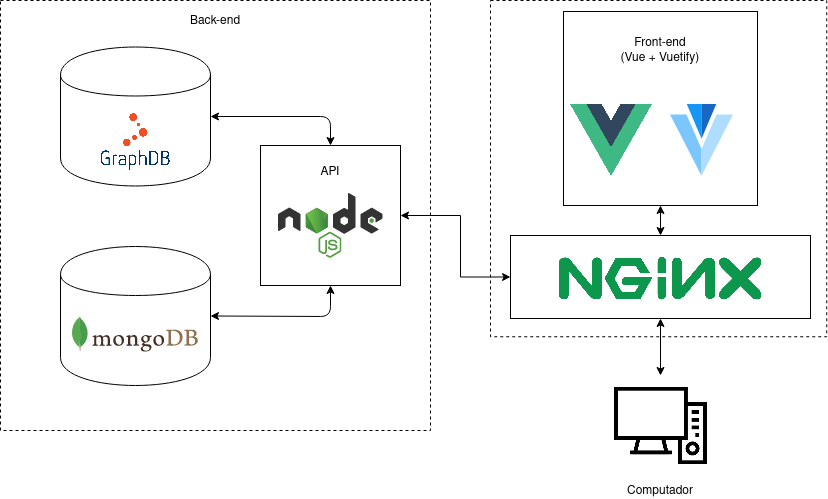
\includegraphics[width=0.7\textwidth]{img/clav_struct2.png}
    \end{center}
    \caption{Estrutura evoluída da \acrshort{clav}}\label{fig:clav_struct2}
\end{figure}

%TODO
TODO: Explicar onde está cada informação: ontologia, utilizadores, classes, etc

\section{Formas de autenticação}\label{sec:autenticacao}
A \acrshort{api} de dados e a interface estavam inicialmente ``juntas'' (aplicação monolítica) onde as rotas eram protegidas contudo, com a separação da aplicação em duas partes, ambas partes deixaram de estar protegidas. Devido à plataforma já ter estado protegida esta já possui duas formas de autenticação, através de chaves \acrshort{api} e através de utilizadores registados. Ou seja, tanto o registo de utilizadores e de chaves API já se encontra implementado bem como o \textit{login} de utilizadores.

As chaves \acrshort{api} existem por forma a dar acesso a certas rotas da \acrshort{api} a aplicações que interajam com a mesma (por exemplo sistemas de informação) sem a necessidade de interação humana.

Já os utilizadores possuem múltiplos níveis de acesso sendo que consoante o seu nível podem ou não aceder a uma rota da interface ou da \acrshort{api}. Os utilizadores podem se autenticar através de \textit{email} e \textit{password} ou com recurso ao \acrfull{cc} através do Autenticação.gov, este último apenas disponível através da interface da \acrshort{clav}.

A hierarquia dos níveis de acesso, do nível que permite menor para o maior acesso, é a seguinte:
\begin{itemize}
    \item Nível 0: Chaves API
    \item Nível 1: Representante Entidade
    \item Nível 2: Utilizador Simples
    \item Nível 3: Utilizador Avançado
    \item Nível 3.5: Utilizador Validador (\acrshort{ad})
    \item Nível 4: Utilizador Validador
    \item Nível 5: Utilizador Decisor
    \item Nível 6: Administrador de Perfil Funcional
    \item Nível 7: Administrador de Perfil Tecnológico
\end{itemize}

As chaves \acrshort{api} poderão aceder a algumas rotas com método \texttt{GET}.
Já os utilizadores poderão realizar todos os pedidos que as chaves \acrshort{api} podem realizar mas quanto maior o seu nível de acesso mais rotas poderão aceder.

A proteção da \acrshort{api} terá de ter esta hierarquia em conta.

\subsection{Registo}

Como já referido, tanto o registo de chaves \acrshort{api} como de utilizadores já se encontra implementado.

Para o registo de uma chave \acrshort{api} é necessário providenciar um nome, um email e a entidade a que pertence. Após o registo da chave a informação desta chave \acrshort{api} é mantida numa base de dados \textit{MongoDB}.

Um utilizador pode se registar através de \texttt{email + password} ou através do Autenticação.gov. No primeiro caso, ao se registar necessita obviamente de indicar o seu email, a \textit{password}, o seu nome, a entidade a que pertence e o nível de acesso que pretende. Já no caso do Autenticação.gov para o registo do utilizador é necessário todos os campos anteriores exceto a \textit{password} (pode ser depois definida), sendo também necessário o campo \acrfull{nic} do utilizador. Caso o registo seja efetuado com recurso à interface do Autenticação.gov apenas será necessário indicar o email, a entidade a que pertence e o nível de acesso que pretende visto que os restantes campos são fornecidos pela Autenticação.gov quando o utilizador se autentica e autoriza a partilha dessa informação com a plataforma da \acrshort{clav}.
A \textit{password} é armazenada não na sua forma literal mas sim a sua \textit{hash} ao aplicar a função criptográfica \texttt{bcrypt}. A utilização de funções de \textit{hash} criptográficas ao armazenar \textit{passwords} impede que as \textit{passwords} originais se saibam caso a base de dados seja comprometida. Para além disso, como o \texttt{bcrypt} combina um valor aleatório (\texttt{salt}) com a \textit{password} do utilizador, é impossível pré-computar a \textit{password} que deu origem ao \textit{hash} sem saber o \texttt{salt}\footnote{Para mais informação veja \textit{rainbow table attack}}.

Durante esta tese com a proteção da \acrshort{api} ficará apenas possível o registo de utilizadores através de utilizadores que já estejam registados e possuam um nível de acesso suficiente para registar utilizadores. Estes utilizadores registados e autorizados pertencem à entidade \acrshort{dglab}. Portanto por forma a utilizadores representantes de outras entidades se registarem na plataforma terão de:~\cite{clavwebpage}
\begin{itemize}
    \item Preencher o formulário disponibilizado para o efeito, para cada representante designado pela entidade;
    \item O formulário deverá ser assinado por um dirigente superior da Entidade e autenticado com assinatura digital, se o envio for feito por via eletrónica (NB\@: não serão aceites assinaturas do formulário por dirigentes intermédios). Esta autorização autenticada pelo dirigente superior é o equivalente a uma delegação de competências, uma vez que o representante da entidade passa a ter capacidade para, em nome da entidade, submeter autos de eliminação, propostas de tabelas de seleção e novas classes para a Lista Consolidada;
    \item O formulário deverá ser remetido à \acrshort{dglab} por via postal ou eletrónica, respetivamente, para:
    \begin{itemize}
        \item \acrshort{dglab}, Edifício da Torre do Tombo, Alameda da Universidade, 1649--010 Lisboa (formulário assinado manualmente) ou
        \item clav@dglab.gov.pt (formulário com assinatura digital).
    \end{itemize}
    \item Após receção do formulário, a \acrshort{dglab} efetuará o(s) respetivo(s) registo(s) até 48 horas úteis;
    \item Findo esse prazo, o utilizador poderá aceder à plataforma, selecionando a opção ``Autenticação'';
    \item A autenticação, no primeiro acesso, deve ser efetuada com o \acrlong{cc}.
\end{itemize}

%TODO
TODO: explicar melhor a parte de autenticacao.gov

\subsection{\textit{Login}}

O \textit{login} apenas está presente para o caso dos utilizadores visto que assim que uma chave \acrshort{api} é registada é enviado por email um \acrshort{jwt} com a duração de 30 dias a ser usado nos pedidos a realizar à \acrshort{api}. O utilizador poderá ao fim dos 30 dias renovar a sua chave \acrshort{api}, onde é gerado um novo \acrshort{jwt}.

Portanto do lado dos utilizadores é possível como já referido realizar o \textit{login} de duas formas através de uma estratégia local ou através do Autenticação.gov.

A estratégia local (\texttt{email + password}) é conseguida através do uso do \textit{middleware} \textit{Passport}.
O \textit{Passport} é um middleware de autenticação para \textit{Node.js} que tem como objetivo autenticar pedidos.~\cite{passport} Tem como única preocupação a autenticação delegando qualquer outra funcionalidade para a aplicação que a usa. Este \textit{middleware} possui muitas estratégias de autenticação entre as quais a local (\texttt{email/username + password}), \acrshort{jwt}, \textit{OAuth}\footnote{Protocolo \textit{open-source} com o objetivo de permitir a autenticação simples, segura e padrão entre aplicações móveis, \textit{web} e \textit{desktop}}, \textit{Facebook} ou \textit{Twitter}. Cada estratégia está num módulo independente. Assim as aplicações que usam o \textit{Passport} não terão um peso adicional devido a estratégias que nem sequer usam.

No caso do \textit{login} através do Autenticação.gov, o utilizador tem de se autenticar na interface do Autenticação.gov (a partir do botão disponível na área de autenticação da interface do \acrshort{clav}). O fluxo do \textit{login} neste caso é:

\begin{figure}[H]
    \begin{center}
        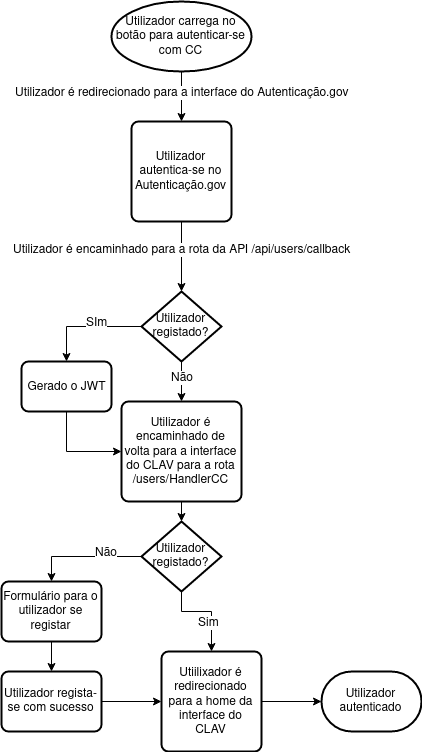
\includegraphics[width=0.5\textwidth]{img/authgov.png}
    \end{center}
    \caption{Fluxo do \textit{login} de um utilizador através do Autenticação.gov}\label{fig:authgov}
\end{figure}

No \textit{login} do utilizador é gerado um \acrshort{jwt} com a duração de 8 horas que deve ser usado nos pedidos a realizar à \acrshort{api}. No fim das 8 horas o utilizador necessita de se autenticar de novo.

%TODO
TODO: explicar melhor a parte de autenticacao.gov
